\chapter{Vizualizační knihovna}\label{sec:Implementation2}

Tato knihovna slouží pro vizualizaci průchodu regulárním výrazem.
Pro získání informací o vyhledávání, slouží již zmíněná knihovna, která byla popsána v předchozí kapitole \ref{sec:Implementation1}.
Hlavním cílem této části aplikace je, na implementovat uživatelsky přívětivé a intuitivní rozhraní.
To umožňuje zadávat regulární výrazy, text ve kterém lze pomocí zadaného výrazu vyhledávat a následnou vizualizaci ve formě debuggeru.

%TODO

\section{Návrh}

Vstupem knihovny HTML soubor \textit{main.html}.
Ten vkládá skript \textit{index.ts}, jehož hlavním účelem je inicializovat vše potřebné pro chod aplikace.
Hlavní třídou, která se stará o obsluhu vizualizace je RegexVisualizer. 
Jejím úkolem je obsluhovat ostatní komponenty a přímo komunikuje s třídou \textit{Regexer} a tím získává data pro vizualizaci.
Pro interakci uživatele slouží dva textové editory, ty jsou ve formě dvou tříd \textit{RegexEditor} a \textit{StringMatchEditor}.
Obsluhují HTML elementy pro zadávání textu, jejich základní funkcionalita je děděna ze třídy \textit{TextEditor}.
Pro samotnou vizualizaci ve formě ladícího nástroje, existuje třída \textit{RegexDebugger}.
Má za úkol, obsluhovat okno aplikace, kde se samotný debugger nachází.
Obsahuje i vlastní posuvník (\textit{Slider}), který dokáže vyvolávat události, s informací o aktuální hodnotě posuvníku.
Také má například možnost automatického přehrávání a změnu rychlosti.

%TODO

%TODO: change loc
\subsection*{Komunikace s třídou regexer}

%TODO

\section{Implementace textových editorů}

Ve vizualizaci se nachází dva textové editory, pro zadávání regulárního výrazu a druhý pro zadávání řetězce, ve kterém proběhne vyhledávání na základě zadaného výrazu.
Jejich funkcionalita je obalena ve dvou třídách, každá sloužící pro jiný textový editor a obě dědí ze třídy \textit{TextEditor}.
Tento vztah lze vidět na obrázku \ref{fig:TextEditor}.

\begin{figure}[!h]
	\centering
	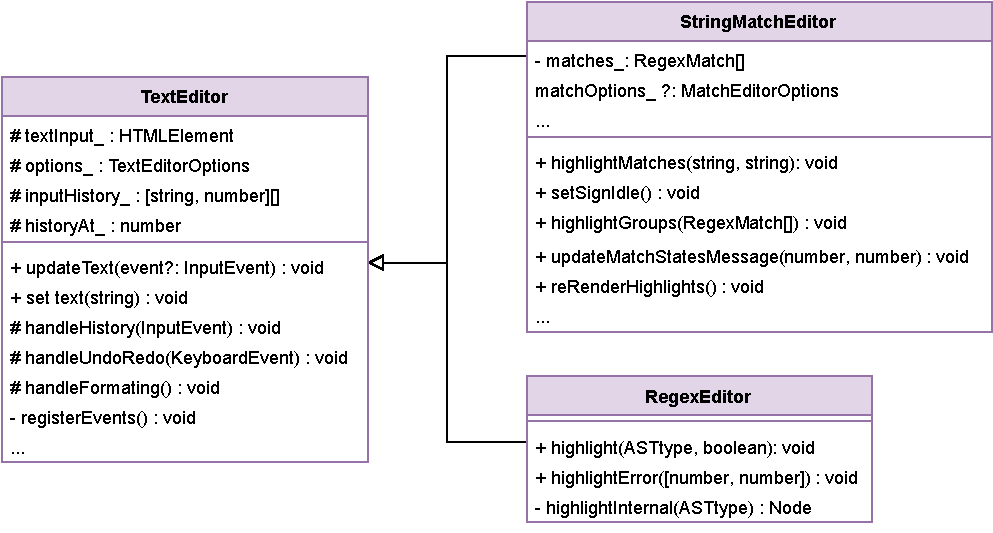
\includegraphics[width=0.8\textwidth]{Figures/TextEditor.pdf}
	\caption{Třídní diagram textových editorů}
	\label{fig:TextEditor}
\end{figure} 

\subsection*{Základní řešení}

Pro řešení textových editorů, jsem se rozhodl pro vlastní implementaci, pro větší flexibilitu a řešení konkrétních problému, týkajících se práce s regulárními výrazy.
Textový editor umožňuje rozšířené možnosti práce s textem, oproti HTML elementům, jako jsou input nebo textarea.
Tyto možnosti jsou například vlastní formátování, nebo správa historie. 
K realizaci samotných vstupů, jsem použil základní obalující HTML blok span.
Na zvoleném bloku tolik nezáleží, ale je potřeba, aby měl atribut \textit{contenteditable}, s nastavenou hodnotou na true.
Tento atribut povoluje psaní přímo do daného bloku. 
Oproti elementu jako je input, lze zde vkládat HTML kód a tím upravovat formátování textu.
To je vhodné pro regulární výrazy, jelikož sami o sobě nejsou moc přehledné.

\textit{TextEditor} slouží jako vzorová třída, pro realizaci textových editorů.
Drží si referenci na HTML element, který obsluhuje, pod názvem \textit{textInput\_}. 
Pro interaktivitu s tímto elementem, je potřeba zaregistrovat různé události.
Mezi ně patří např. psaní, mazání, undo a redo. 
Události jsou registrovány při vytvoření instance třídy, pomocí soukromé metody \textit{registerEvents}.
Pokud je zavolána, chráněná metoda \textit{handleFormating}, tak dojde ke změně podoby textu na formátovanou.
Jedná se o grafické zobrazení bílých znaků, jako je nový řádek nebo tabulátor.

%TODO
% TODO: mby add element helper

\subsection*{Zvýraznění syntaxe}

Součástí třídy \textit{RegexEditor}, je metoda sloužící pro zvýrazňování syntaxe regulárních výrazů. 
Pro zvýraznění slouží získaná AST struktura po dokončeném parsování.
Algoritmus řešení tohoto problému, funguje na principu rekurzivního zanoření, ve stromové struktuře.
Každý symbol, který má být zvýrazněný, je obalený v HTML bloku, s třídou identifikující o jaký symbol se jedná.
U jednotlivých vzorů, záleží na pořadí zpracování symbolů a rekurzivního zanoření.
Například skupina, se zpracovává tak, že první se zvýrazní otevírací závorka "(".
Poté se algoritmus rekurzivně zanoří, nebo-li zpracuje potomky (vnitřní část) skupiny a nakonec zvýrazní ukončující závorku ")".
Výsledkem vznikne HTML struktura, která popisuje symboly a vzory regulárních výrazů.
Tyto symboly jsou pak zvýrazněny, pomocí různých barev, definovaných v CSS.

\subsection*{Historie}
Práci s historii jsem musel na implementovat vlastní, jelikož původní nefungovala správně.
Důvodem bylo časté přepisování textu, z již zmíněného formátování.
Aby historie fungovala, musel jsem vytvořit pole, které obsahuje jak původní řetězec tak pozici kurzoru v něm.
Pokud byla vyvolána operace vrácení se zpět v historii (undo), překopíruje se uložený řetězec do textového pole a kurzor se nastaví na správnou pozici.
K odstranění záznamu z historie nedochází, jelikož může být vyvolána \textit{redo} operace, nebo-li odvolání operace \textit{undo}.
Pokud dojde k uložení nového stavu textového pole, tak všechny stavy za ukazatelem se smažou a přidá se zde nový.
V nastavení editoru, jsem přidal možnost zvolit si maximální počet záznamů v historii.
Pokud ale není nastavená, automaticky se omezí na 100 záznamů.

\subsection*{Pozice kurzoru}
Práce s textovým kurzorem je další značná část textových editorů.
Pokud uživatel píše do textového pole, často nastává ke změně textu na pozadí samotnou aplikací.
Například při zvýraznění, dochází ke změně textové formy na HTML strukturu.
Při změně vždy dojde k resetování pozice kurzoru v textu.
To ale pro uživatele není příjemná vlastnost, kterou jsem tedy musel vyřešit.

Před přepsáním textového pole, je uložená pozice kurzoru.
Po vložení textu, je nutné vrátit se na uloženou pozici. 
Nejedná se ale o jednoduchou úlohu, jelikož pokud se v textu nachází HTML elementy, musí být brány v potaz.
Použil jsem základ algoritmu ze stránky \textit{stackoverflow}\footnote{https://stackoverflow.com/questions/69956977}, který dokáže jak zjistit aktuální pozici kurzoru, tak z pozice umístit kurzor na správné místo.
Ten jsem upravil pro potřeby mého projektu a dále rozšířil.
Například jsem přidal možnost vytvoření nového kurzoru, který není přímo vložený do dokumentu, což se může hodit pokud je potřeba získat souřadnice písmena.

\section{Vizualizace průchodu}

Vizualizace ve formě debuggeru je obsluhována třídou \textit{RegexDebugger}.
Okno pro vizualizaci se otevře po kliknutí na tlačítko, které je předáno třídě součástí konstruktoru.
Debugger obsahuje identická pole jako textová pole pro interakci s uživatelem, avšak již nelze jejich text editovat.
Dále disponuje posuvníkem, který slouží pro procházení průběhu vyhledávání. 

\subsection*{Posuvník}

Posuvník jsem zvolil, jako jednoduchou a intuitivní možnost procházení historie.
Jeho implementace je ve vlastní třídě a jeho součástí je nastavení, pro příjemnější manipulaci výsledného posuvníku.
Pomocí nastavení, lze vypínat/zapínat některé funkcionality, nebo měnit samotný vzhled, jako je barva či velikost.
Tato realizace je vlastní, z důvodu lehčí integrace do aplikace.

Při vytváření instance této třídy, musí být předán HTML element nebo id elementu, do kterého se posuvník vykreslí.
Nastavení je dobrovolné, pokud není předáno zvolí se základní.
Posuvník může mít tlačítka pro ovládání, těmi jsou automatické přehrávání, vpřed, zpět, na konec a na začátek.
Pro automatické přehrávání, může být součástí pole, pro editaci rychlosti, pokud je povolené v nastavení.

Posuvník může pouze nabývat celo-číselných hodnot, v omezeném rozmezí od min do max.
Pokud se změní jeho hodnota, je vyvolána vlastní událost, která tuto hodnotu obsahuje.
Ta může být odchycena, např. jinou třídou.

\subsection*{Zvýraznění pozice a backtrackingu}

\section{Uživatelské rozhraní}

\subsection*{Využití VScode stylů}

\subsection*{Ovládání aplikace}

\endinput